\chapter{Theoretical Background}

\section{Feature Engineering}

Data mining is a machine learning tool that uses statistical methods to discover patterns in large data sets. Data mining has various stages to process knowledge and all of the stages run different methods to collect the appropriate data.\medskip

The first and most important part is to select the dataset which will be processed. This implies the following: Firstly the goal needs to be cleared up. Secondly the information that seems to be useful for the goal needs to be selected. \medskip

\noindent To decide the usefulness of a feature, it should pass the some quality requirements.
\begin{verse}
	$\bullet$ Validity: the degree to which the measures conform to defined business rules or constraints\\
	$\bullet$ Accuracy: the degree of conformity of a measure to a standard or a true value\\
	$\bullet$ Completeness: the degree to which all required measures are known\\
	$\bullet$ Consistency: the degree to which a set of measures are equivalent in across systems\\
	$\bullet$ Uniformity: the degree to which a set data measures are specified using the same units of measure in all systems
\end{verse}

There are some other criteria for the qualities of good features. A useful feature vector value appears more than one times in a data set, which enables the model to learn the relationships between the feature vector values and the associated labels. This means having many examples with the same value helps the model to see the feature in different settings to determine when it is a good predictor. Also, each feature should have a clear and obvious meaning.


\subsection{Data Mining}

\textbf{Data preprocessing} \cite{pyle1999data} is a data mining technique that involves transforming raw data into an understandable format. The selected dataset may include errors, missing values or noisy, inconsistent data which have to be filtered during the preprocessing stage. \medskip

Data preparation and filtering steps can be time consuming. Data preprocessing includes cleaning, integration and reduction. Sometimes data transformation takes place in the preprocessing too. The product of data preprocessing is the final training set.\bigskip

The given data in large datasets often contains information that is not clear enough. There are several techniques for repairing these uncertain data. \bigskip

\noindent For resolving missing values, the following steps can be taken:\\
1. Simply remove the feature vector, which is only effective if the vector contains several missing attributes.\\
2. Fill the missing values manually, which can be done with the mean value.\\
Both techniques can create noise and inaccuracy, but it is important to deal the appropriate technique, because the incorrect feature vector may contain necessary information too. \bigskip


Noise is a random error or variance in a measured variable. Noisy data needs to be smoothed to get the accurate prediction. Binning methods smooth the value with its neighbour's, so it is just a local smoothing technique. Clustering can be used to detect outlier values by organizing them into similar groups. Data can be smoothed by fitting a function like regression to the data.\medskip

Data inconsistencies can be solved manually by external references, or with the use of knowledge engineering. In the known of the meaning of every feature, it can be obvious to recognize an inconsistent value manually. Knowledge engineering uses technical, scientific and social aspects to deal with a feature value's inconsistency.\medskip


Data integration and reduction aims on the same goal, which is to make the dataset smaller. During integration, an algorithm is looking through the dataset and looking for redundacies and multiple data. \medskip

Data reduction is reducing the volume or the dimension of the dataset, without compromising the integrity of the original dataset. As the analysing can be time consuming, these data reduction techniques are really helpful in large datasets:\\
1. Dimension reduction: drop the irrelevant or weakly relevant values from the dataset\\
2. Data compression: use various encoding techniques to reduce the size of the dataset


\subsubsection{Transformation and Feature Scaling}

Some features of the dataset need to be transformed to get an appropriate form for data mining. Data transformation has a strong connection with \textbf{feature scaling} \cite{zheng2018feature}\cite{dong2018feature}, which is a statistical method used to standardize the range of the data. Feature scaling uses mathematical procedures to scale the range. 

\begin{figure}[h]
	\centering
	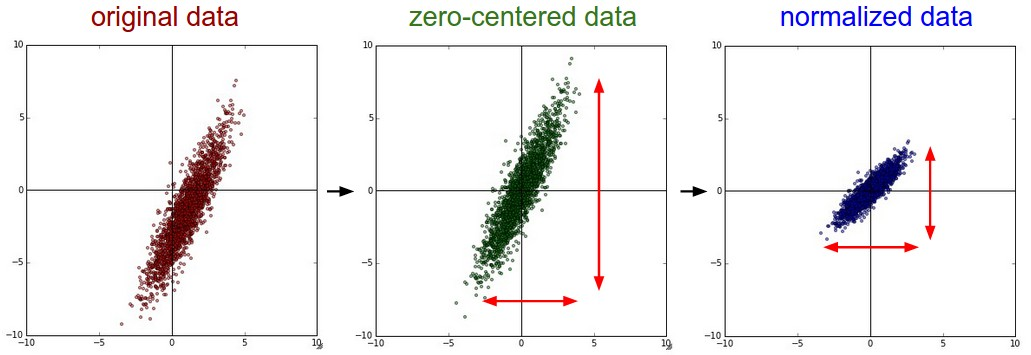
\includegraphics[height=0.35\linewidth]{./figures/data_mining}
	\caption{Data mining techniques can be used to convert data into understandable form.}
	\label{fig:data_mining}
\end{figure}

\textbf{Normalization} is the process of scaling individual samples to have a unit norm. Min-max scaling is the simplest normalization method that rescales the features to a range of $[0, 1]$ or $[-1, 1]$. The selected range depends of the data. It can be written as the following \eqref{eq:min-max}, where $x$ is the original, and $x'$ is the normalized value:
\begin{equation} x' = \frac{x-min(x)}{max(x)-min(x)} \label{eq:min-max} \end{equation} 

\smallskip \noindent Mean normalization \eqref{eq:mean} is similar to min-max scaling, where $\bar x$ is the mean of $x$:
\begin{equation} x' = \frac{x-\bar x}{max(x)-min(x)} \label{eq:mean} \end{equation} \medskip

\textbf{Standardization} is the process to transform the given data as if they comes from standard normally distributed data set. Feature standardization \eqref{eq:standard} makes the values of each feature to have zero-mean and unit-variance. 
\begin{equation}  x'= \frac{x-\bar x}{\sigma} \label{eq:standard} \end{equation}
where $x$ is the original feature vector, $\bar x$ is the mean of that feature vector and $\sigma$ is its standard deviation.\bigskip

\textbf{Encoding} is the process of converting data into an acceptable form for information processing. It can be used effectively on categorical features, because they just use a set of values. \smallskip

Integer encoding converts the nominal values to numeric values. These numeric values are integers in increasing order, and they can cause inconsistency with the given weights.\smallskip

One-hot encoding offers a solution for the inconsistency problem. It creates a binary vector for each categorical feature in the dataset where the values appears as follows:\\
$\bullet$ For those values, which apply to the example, set the vector values to 1.\\
$\bullet$ Set other values to 0.\\
The length of the binary vector is equal to the number values in the current feature.


\subsubsection{Data Mining Algorithms}

As mentioned, the product of data mining is the training set. For the application of data mining algorithms, the original data set is usually split into multiple sets. There are two data sets, which are separated during the creation of the model. The first one is called \textbf{training set}, which is used by the machine learning algorithm to gather knowledge and increase accuracy. The other one is the \textbf{testing set}, which is used to provide a data set to test function estimation accuracy of the learning algorithm on the training data set.\medskip

After the split, the following data mining techniques \cite{pujari2001data} can be used on the training set to discover the patterns:\\
1. Classification: This method helps to retrieve information by classifying data into different classes. It can be use to draw further conclusions.\\
2. Clustering: It can be used to identify data which are similar to each other. It is an effective way to understand the similarities and differences between values.\\
3. Regression:  This method analyzes the relationship between variables, to determine desired unknown values.\\
4. Association: It can discover hidden patterns in the dataset by identifying special events, for example high correlations between values.\\
5. Outer detection: It collects outlier values which do not match an expected pattern or expected behavior. \\
6. Sequential Patterns: This method helps to identify similar patterns for a certain period. \\
7. Prediction: This method can be used for predicting future values in a dataset with the known of the given data and past events.  \medskip

The techniques of data mining originates from a wider field called \textbf{data analytics}. In a simple explanation, data analytics is the process of examining data sets in order to draw conclusions about the information they contain. It focuses on processing and performing statistical analyzis on existing data sets. A widely used data analytics technique is machine learning.



\section{Single-Layer Perceptron}

The perceptron is a single layer feedforward neural network \cite{tho2010perceptron}, which has only one input and output layer. The input values are presented to the perceptron, and if the predicted output is the same as the desired output, then the performance is considered satisfactory and no changes to the weights are made. However, if the output does not match the desired output, then the weights need to be changed to reduce the error. \medskip

In order to avoid unnecessary iterations, it is important to adjust the weights \eqref{eq:slp} properly.
\begin{equation} \Delta w = \eta * d * x \label{eq:slp} \end{equation} 
where $\Delta w$ stands for the current weight, $\eta \leq 1$ is the learning rate which is the size of the required steps, $d$ represents the desired output and $x$ is the input data.\medskip

A single-layer perceptron's units are the artificial neurons, that are conventionally called \textbf{nodes}. To determine the value of a node, all the inputs would be multiplied by their respective weights, and then summed. This weighted sum stands for \textbf{dot product} in this context: $ z = w_1 x_1 + w_2 x_2 + \dots + w_m x_m = \sum_{j=1}^m w_j x_j $

\begin{figure}[h]
	\centering
	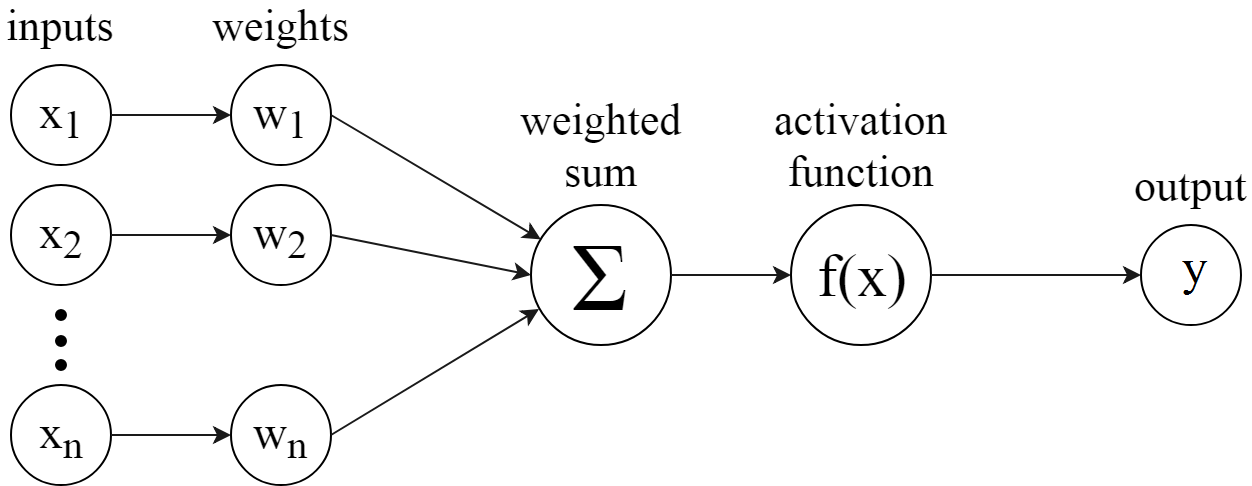
\includegraphics[height=0.28\linewidth]{./figures/perceptron}
	\caption{The appropriate weights are applied to the inputs and the resulting weighted sum passed to an activation function that produces the output.}
	\label{fig:perceptron}
\end{figure}

The output $o$ in \eqref{eq:slp-output} is determined by whether the weighted sum $\sum_j(w_j x_j)$ is less than or greater than some threshold value $\theta$, which is the parameter of the neuron. If that value is above a given threshold, it "fires", which means that the neuron gets an activated value. 
\begin{equation} o = \begin{cases} 0, & \hbox{for}~ \sum_j(w_j x_j) < \theta \\ 1, & \hbox{for}~ \sum_j(w_j x_j) \geq \theta \end{cases} \label{eq:slp-output} \end{equation} 



\section{Feedforward Neural Networks}

The feedforward neural network \cite{fine2006feedforward} is a type of neural networks, which aims to create a mapping from a properly trained input dataset to an estimated output. This type of neural network is called feedforward as there are no feedback connections in which outputs of the neuron are connected to itself. A feedforward neural network is able to model complex non-linear functions. \medskip

A typical feedforward neural network consists of input and output layers. There is an intermediate part between inputs and outputs, called hidden layers. The \textbf{input layer} is a set of input neurons, where each neuron represents a feature in our data set. The \textbf{output} of any feedforward network is the sum of the inputs multiplied by the weights. The \textbf{hidden layer} contains units which can transform the inputs into a mapping that the output layer can use. The relationship between the input and hidden layer is determined by the weights of the network. \medskip

\noindent The output of a trained feedforward neural network can be characterized by \eqref{eq:feedforward}
\begin{equation} o_k = f_k(i,w) \label{eq:feedforward} \end{equation}
where $o_k$ is the $k$th neural network output, $(i,w)$ is a vector of the weights and $f_k(\cdot)$ describes the mapping from the input to the $k$th output, where $f_k(\cdot)$ also contains the structure of the feedforward perceptron. The neural network can be trained if the input and the output are fixed and the weights are set. When a single scalar output can be found, $o_k$ can be replaced by $o$ and $f_k(\cdot)$ by $f(\cdot)$.



\subsection{Multi-Layer Perceptron}

The multi-layer perceptron is a multi-layered feedforward neural network algorithm that learns a function $f(\cdot) : \mathbb{R}^m \mapsto \mathbb{R}^o$ by training on a dataset, where $m$ is the number of dimensions for input and $o$ is the number of dimensions for output. Given a set of features $X = x_1, x_2, \dots, x_m$ and a target $y$, it can learn a non-linear function approximator for either classification or regression. \medskip

The difference between single- and multi-layered neural networks is that the multi-layered perceptron has one or more hidden layers besides the input and output layer. Except for the input nodes, each node is a neuron that uses a linear or non-linear activation function. \medskip

In a multi-layer perceptron, each neuron in one layer is connected with a weight to another neuron in the next layer. Each of these neurons stores a value, which is in general a sum of the weighted neurons which comes from previous layers. There is a special unit, called \textbf{bias}, that are not influenced by any values in the previous layer, so they do not have any incoming connections. However they have outgoing connections and they can contribute to the output of the artificial neural network. Bias units stores a constant value, which helps the model to fit the best for the given data. Hence the definition of dot product expands like this \eqref{eq:mlp}:
\begin{equation} z = \sum_{j=1}^m w_j x_j + bias \label{eq:mlp} \end{equation}

Neural networks are designed to learn from datasets using iterative methods. Estimation value error is calculated from the estimated and the measured values to modify the weights of the connections between neurons. 
A multi-layer perceptron utilizes a supervised learning technique called \textbf{backpropagation} for training.


\subsubsection{Backpropagation}

The main goal of backpropagation \cite{chauvin2013backpropagation} is to update all of the weights in the neural network, in such way that the predicted output to be closer to the target output with minimizing the error of each output neuron and also the network.

The algorithm consists of two phases: the forward phase where the activations are propagated from the input to the output layer, and the backward phase, where the error between the actual and the desired value in the output layer is propagated backwards to modify the weights values. \medskip

The function that is used to compute this error is known as \textbf{loss function}. For backpropagation, the loss function calculates the difference between the network output and its expected output, after a training example has propagated through the network. \medskip

Different loss functions will give different errors for the same prediction, and thus have a considerable effect on the performance of the model. In the training of multi-layer perceptrons, L2 loss function $L$ has been used in \eqref{eq:backprop}, which is the square of the L2 norm of the difference between actual value $y$ and predicted value $\hat{y}$.
\begin{equation} L = \sum^n_{i=1}(y - \hat{y})^2 \label{eq:backprop} \end{equation}



\subsubsection{Gradient descent}

Backpropagation uses gradient descent \cite{anderson1995introduction} in the calculation of the weights. It is an optimization method, which aims on to minimize a given function to its local minimum by iteratively updating the weights of the model. The input is defined with an initial value and the algorithm calculates the gradient i.e. the partial derivative of the loss curve at this starting point. \medskip

\noindent The components of gradient descent are the following:
\begin{verse}
	$\bullet$ Learning rate: size of steps took in any direction\\
	$\bullet$ Gradients: the direction of the steps, i.e. the slope\\
	$\bullet$ Cost function: tells the current height, which is the sum of squared errors
\end{verse}

\begin{figure}[h]
	\centering
	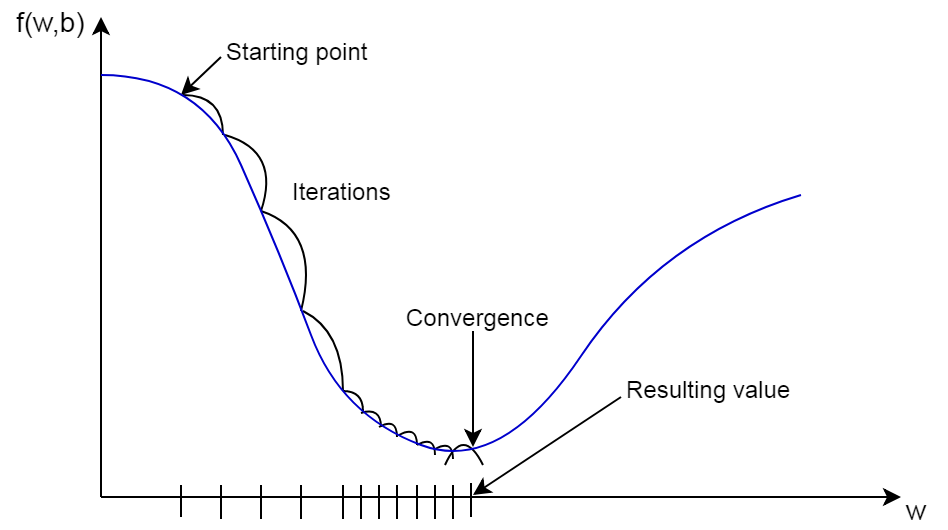
\includegraphics[height=0.35\linewidth]{./figures/gradient}
	\caption{The gradient descent is an optimization method used by backpropagation}
	\label{fig:gradient}
\end{figure}

In backpropagation, the calculation of the gradient passes the network backwards, so the values of the gradient from one layer are reused in the computation of the gradient for the previous layer. 



\section{Training a MLP Model}

The task that is being tackled in this paper is to make the inversion of a single element feedforward neural network. To eventuate this successfully, the appropriate dataset is given and already preprocessed. Hence the main task is now to train a neural network to predict new outputs for the testing set and minimize the loss between the given and the desired outputs from the training set. \medskip

The components of a neural network model i.e the activation function, optimization algorithm and the size of the layers play a very important role in effectively training a model and produce accurate results. Different tasks require a different set of functions to give the most optimum results. The used methods and functions are described in the following subsections.


\subsection{Regression}

Regression \cite{allen2007understanding} is a supervised learning task of machine learning that is used to predict values of a desired target variable. It is a statistical technique which requires a data set with the desired output that is consists of one or more continuous variables and real numbers.\smallskip

By using regression the input vector is mapped onto a given set of values by the network. The network regresses the independent variables, provided by the inputs, onto the dependent variable. The multi-layer perceptron uses non-linear regression while trying to approximate the values of the dataset.

\begin{figure}[h]
	\centering
	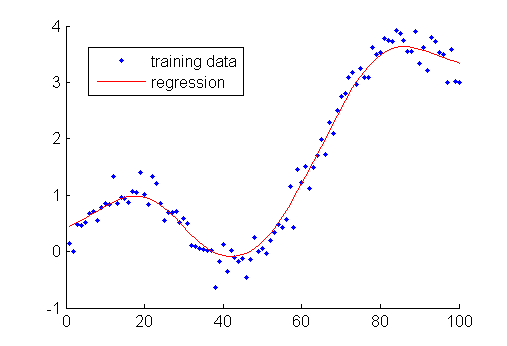
\includegraphics[height=0.4\linewidth]{./figures/regression}
	\caption{Regression is used to find the best fit of the training
		data}
	\label{fig:regression}
\end{figure}


\subsection{Activation Functions}

In connection with artificial neural networks, the activation function is a transitional state of the neurons between other layers. It is a mapping of the previous layers and it maps the resulting value into the desired range, which is usually between -1 and 1. The output of the activation function is then used as input for the next layer, until a desired solution is found. There are several activation functions, and each of them utilizes different methods for mapping. \medskip

As the multi-layer perceptron approximates non-linear functions, it will be the most accurate by using non-linear activation functions as well \cite{pillo2013nonlinear}. These non-linear activation functions are known about having more than one degrees and they have a curve in their graph. As non-linear functions can generate non-linear mappings from inputs to outputs, they can be applied on complex data sets. 

\begin{figure}[h]
	\centering
	\caption{The graphs of the most popular non-linear activation functions}
	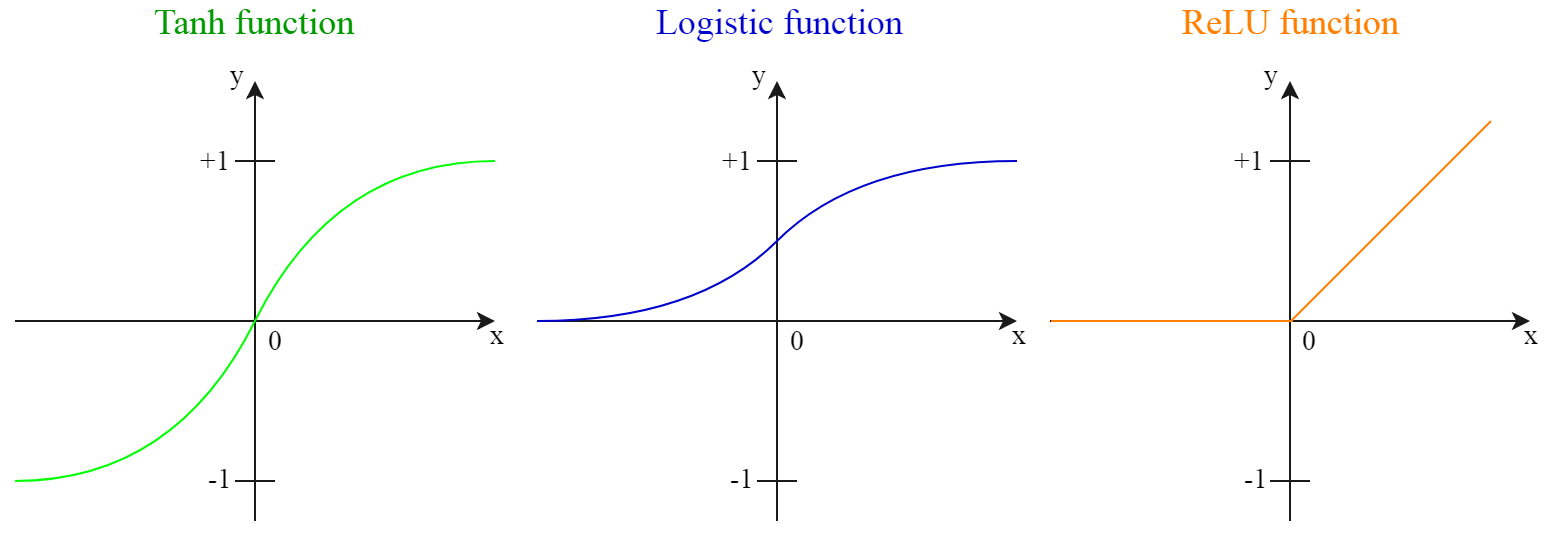
\includegraphics[height=0.35\linewidth]{./figures/functions}
	\label{fig:functions}
\end{figure}

\bigskip \noindent The two common non-linear activation functions are both sigmoids, and described by \eqref{eq:activation}
\begin{equation} f(x)=tanh(x) ~~~ \hbox{and} ~~~ f(x)=\sigma (x)=\frac{1}{1+e^{-x}} \label{eq:activation} \end{equation}
The first is a \textbf{hyperbolic tangent} that ranges from -1 to 1, while the other is the \textbf{logistic} function, which is similar in shape but ranges from 0 to 1. \smallskip

The \textbf{ReLU} function is another type of non-linear functions, which stands for rectified linear unit. It is called half-rectified, because no negative values are allowed. This operation affects the resulting graph (\autoref{fig:functions}), as the negative values are shown as zeros \eqref{eq:activation2}.
\begin{equation} f(x) = max(0,X) \label{eq:activation2} \end{equation}



\subsection{Optimization Methods}

Artificial neural networks have different phases in the process of their operation. The learning process in a neural network uses different training methods with different characteristics and performance. These training methods use optimization algorithms to update weights and biases i.e. the internal parameters of a model to reduce the error. \cite{veerarajan2007numerical}\cite{pillo2013nonlinear}\cite{sathasivam2003optimization}



\subsubsection{Stochastic Gradient Descent}

Stochastic gradient descent is a stochastic approximation of gradient descent optimization, used effectively in large-scaled data sets. It can also work in a system of linear and non-linear equations and can effectively solve unconstrained optimization problems. In contrast to gradient descent, the stochastic method can approximate the true gradient of the cost function because it updates the parameters for each training example, one by one. To demonstrate assume that $\eta$ is the learning rate, $L$ stands for the loss function and $\nabla_w L = \frac{\partial L}{\partial w}$ is the gradient. Now the updating equation of the weights $w$ in each iteration is:
\begin{equation} w_{t+1} = w_t - \eta \nabla_w L \label{eq:sgd} \end{equation} 

\begin{figure}[h]
	\centering
	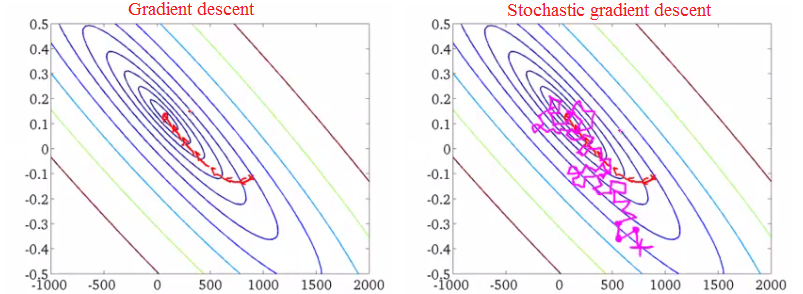
\includegraphics[height=0.28\linewidth]{./figures/stochastic}
	\caption{The difference between the process of GD and SGD methods}
	\label{fig:stochastic}
\end{figure}

\noindent The process of the stochastic gradient descent algorithm is the following:\\
1. Choose one sample from the dataset (this is what makes it stochastic gradient descent).\\
2. Calculate all the partial derivatives of loss with respect to weights or biases. \\
3. Use the update equation \eqref{eq:sgd} to update each weight and bias.\\
4. Go back to step 1.


\subsubsection{Adaptive Moment Estimation}

Another method is adaptive moment estimation, called Adam. It is a transition between adaptive methods and momentum-based methods. In the algorithm, running averages of both the gradients and the second moments of the gradients are used, which means Adam not only stores the exponentially decaying average of past squared gradients $v_t$, it also keeps the decaying average of past gradients $m_t$, similarly to momentum-based methods. The algorithm computes the decaying averages of past $m_t$ and past squared $v_t$ gradients respectively as follows in \eqref{eq:adam1}:
\begin{equation} m_t = \beta_1 m_{t-1} + (1-\beta_1)L_t ~~~~\hbox{and}~~~\ v_t = \beta_2 v_{t-1} + (1-\beta_2)L^2_t \label{eq:adam1} \end{equation}
where $m_t$ and $v_t$ are the estimates of the first and second moments, $\beta_1$ and $\beta_2$ are the decay for gradients and second moments of gradients, and $L_t$ is the loss function.\\
The first and second moment estimates are in \eqref{eq:adam2}:
\begin{equation} \hat{m_t} = \frac{m_t}{a-\beta^t_1} ~~~~\hbox{and}~~~ \hat{v_t} = \frac{v_t}{a-\beta^t_2} \label{eq:adam2} \end{equation}
Then these estimates are used to update the parameters $w$ with a simple scalar $\epsilon$ to prevent division by 0 in \eqref{eq:adam3}:
\begin{equation} w_{t+1} = w_t - \frac{\mu}{\sqrt{\hat{v_t}}+\epsilon}\hat{m_t} \label{eq:adam3} \end{equation}


\subsubsection{Limited-memory BFGS}

Limited-memory BFGS is an approximation of Broyden–Fletcher–Goldfarb–Shanno (BFGS) algorithm, which is an iterative method for solving unconstrained non-linear optimization problems. The difference between them, that L-BFGS uses a limited amount of computer memory. L-BFGS aims on parameter estimation, and the target problem is to minimize $f(x)$ over unconstrained values of the real-vector $x$ where $f$ is a differentiable scalar function. In this method, the Hessian matrix of second derivatives is not computed, but it is approximated by using gradient evaluation updates. \medskip

\noindent From an initial guess $x_0$ and an approximate Hessian matrix $B_0$, the following steps are repeated as $x_k$ converges to the solution:\\
1. Obtain a direction $p_k$ by solving $B_k p_k = - \nabla f(x_k). $ \\
2. Perform a one-dimensional optimization to find an acceptable stepsize $\alpha_k$ in $p_k$. \\
3. Set $s_k = \alpha_k p_k$ and update $x_{k+1} = x_k + s_k.$ \\
4. Set $y_k = \nabla f(x_{k+1}) - \nabla f(x_k).$ \\ 
5. The solution is $B_{k+1} = B_k + \frac{y_k y^T_k}{y^T_k s_k} - \frac{B_k s_k s^T_k B_k}{s^T_k B_k s_k}.$

\begin{figure}[h]
	\centering
	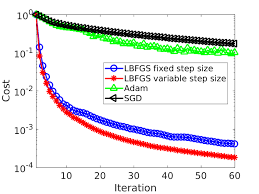
\includegraphics[height=0.34\linewidth]{./figures/optimization}
	\caption{The optimization of SGD, Adam and L-BFGS with respect of cost and iteration}
	\label{fig:optimization}
\end{figure}



\section{Inversion}

The inverse function means the reverse of another function in mathematics. For a given $f: X \mapsto Y$, the inverse function of $f$ is that $g: Y \mapsto X$, where $f(x) = y$ and $g(y) = x$. Thus $g = f^{-1}$. Not all of the functions have inverse functions. A function $f$ has an inverse function, if it is accomplished for every $y$ in $Y$ that there must be one, and only one $x$ in $X$ so that $f(x) = y$.\medskip

Inversion of a neural network consists of clamping the weights and the neural network output while adjusting the input in the neural network until an equality or a best possible fit occurs for one or more values of the input. \medskip

Feedforward neural networks aim on to capture system mapping from the given training data. The goal is to find the input values that will result the desired output for the given weights. Generally it can be determined that a single input can generate numerous outputs. 

\bigskip \noindent The process of finding the inversion $f^{-1}(x)$ of a function $f(x)$ is the following:\\
1. First, replace $f(x)$ with $y$.\\
2. Replace every $x$ with a $y$ and replace every $y$ with an $x$. \\
3. Solve the equation from Step 2 for $y$. \\
4. Replace $y$ with $f^{-1}(x)$. 



\subsection{Single Element Inversion Methods}

In the task of single element inversion only one point is found by the algorithm depending on the initialization. This means it will result a nearer outcome in further processes. Hence it is very important to find a properly training algorithm, because it notes the previously founded points and reuses them. The process of finding the best estimator is time consuming. As the quantity of parameter combinations increases during the training phase, so does the time that the training takes. However, the number of parameter combinations also potentionally increase the inversion accuracy.\bigskip

To solve the inversion of an unconstrained optimization problem, the inversion method needs to solve the optimization itself in its training phase. After the dataset is properly trained, the inversion problem is the following:\medskip

Given some network function $f : X \mapsto Y$, for some $y \in Y$, the appropriate $x \in X$ needs to be found, such that $f(x) = y$. Or more generally, if $L : Y \mapsto \mathbb{R}$ is the loss function defined over the network output, an input $x$ have to be found that minimizes $L(f(x))$. 


\subsection{Williams-Linder-Kindermann Inversion}

\label{para:wlk-inv}The WLK inversion was named after R. L. Williams, A. Linder and J. Kindermann \cite{KINDERMANN1990277}, who firstly introduced the single element search method for inversion of real valued neural network. In this algorithm, the inversion problem is set up as an unconstrained optimization problem and solved by gradient descent, similarly to backpropagation. \medskip

\noindent The method of WLK inversion involves two main steps: \\
1. computing the deltas for every value \\
2. updating the weights manually\medskip

During the training, the neural network is trained to learn a mapping from input to output. The proper set can be find by minimizing the loss. Thus the neural network learns a functional relationship between the inputs and the outputs. Now all the weights are fixed. \medskip

Assume that the initial input vector $i_0$ is given. Now the recursive equation of the training phase is the following: 
\begin{equation} i_k^{t+1} = i_k+t - \eta \frac{\partial E}{\partial i_k^t} \label{eq:wlk} \end{equation} 
$t$ - the index of the iteration, \\
$i_k^t$ - the $k$th component of the $i^t$ vector, \\
$\eta$ - the learning rate \bigskip

Because of the general feedforward topology, the iteration for inversion in \eqref{eq:wlk} can be solved by the derivative of \eqref{eq:wlk_delta}
\begin{equation} \frac{\partial E}{\partial i_k} = \delta k ~~~~ k \in I \label{eq:wlk_delta} \end{equation}
for every $\delta k$ in \eqref{eq:wlk_forward}:
\begin{equation} \delta j = \begin{cases} \varphi'_j(o_j)(o_j-t_j):, & ~ j \in O \\ 
\varphi'_j(o_j)\sum_{m\in H,O}\delta_j w_{jm}:, & j \in I, H \end{cases} \label{eq:wlk_forward} \end{equation}

\noindent $I, O, H$ - the set of input, output and hidden neurons,\\
$w_{jm}$ - the weight value from neuron $j$ to neuron $m$,\\
$\varphi'_j$ - the derivative of the $j$th neuron squashing function,\\
$o_j$ - the activation of the $j$th neuron,\\
$t_j$ - the desired output of the $j$th neuron \bigskip

The derivatives of the neurons need to be solved by backward order from the output to the input.

